\section{Interactions}
This section covers the interactions between the different actors and the applications. Each Subsection will introduce an interaction in more detail.

\subsection{Buy a Ticket}
Figure \ref{fig:buyticket-sequence-diagram} shows the process, when a guest buys a ticket. Hereby, the guest interacts with the guest-client to buy a ticket. The client then sends the requests to buy a ticket to the event SC. The contract updates the owner of the bought ticket and locks the price in ETH until the event has passed. After the event, the host can request to receive the now unlocked ETH from SC to initiate the payment. This step is necessary, since a SC cannot initiate a transaction itself.
\begin{figure}[H]
    \centering
    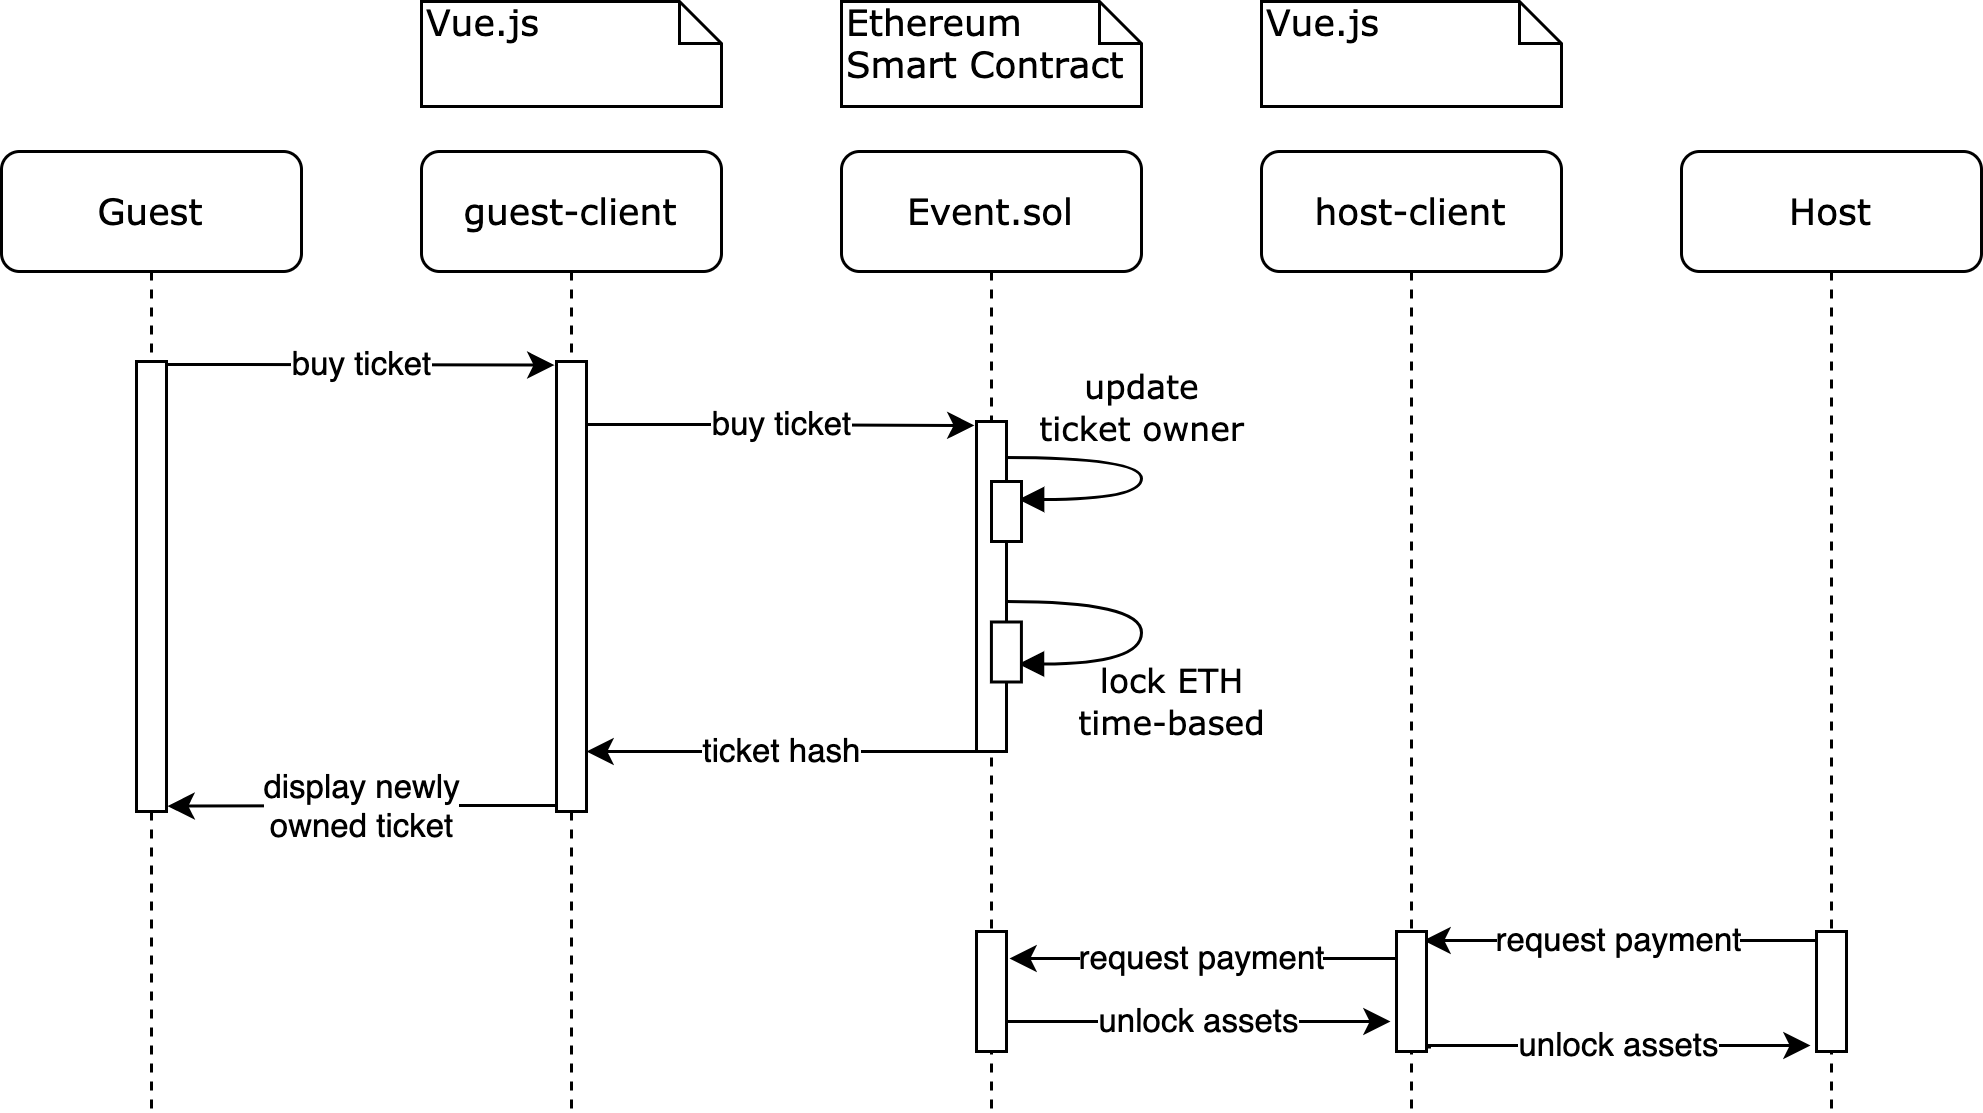
\includegraphics[width=16cm]{design/diagrams/BuyTicket.png}
    \caption{Ticket Sale Sequence Diagram}
    \label{fig:buyticket-sequence-diagram}
\end{figure}

\subsection{Presale}
The sequence diagram in Figure \ref{fig:presale-seuquence-diagram} illustrates how a guest can participate in a ticket presale. When registering for the presale, the ticket price is locked in the SC. The user has the option to opt-out at any time and get the locked ETH back. The event host decides when the presale ends. After this defined end time, the Event SC uses a source of randomness to determine the winners of the presale (see section\ref{section:imp:presale}). If a guest is part of the winners, he can mint his ticket. If not, the guest can claim the spent ETH back.

\begin{figure}[H]
    \centering
    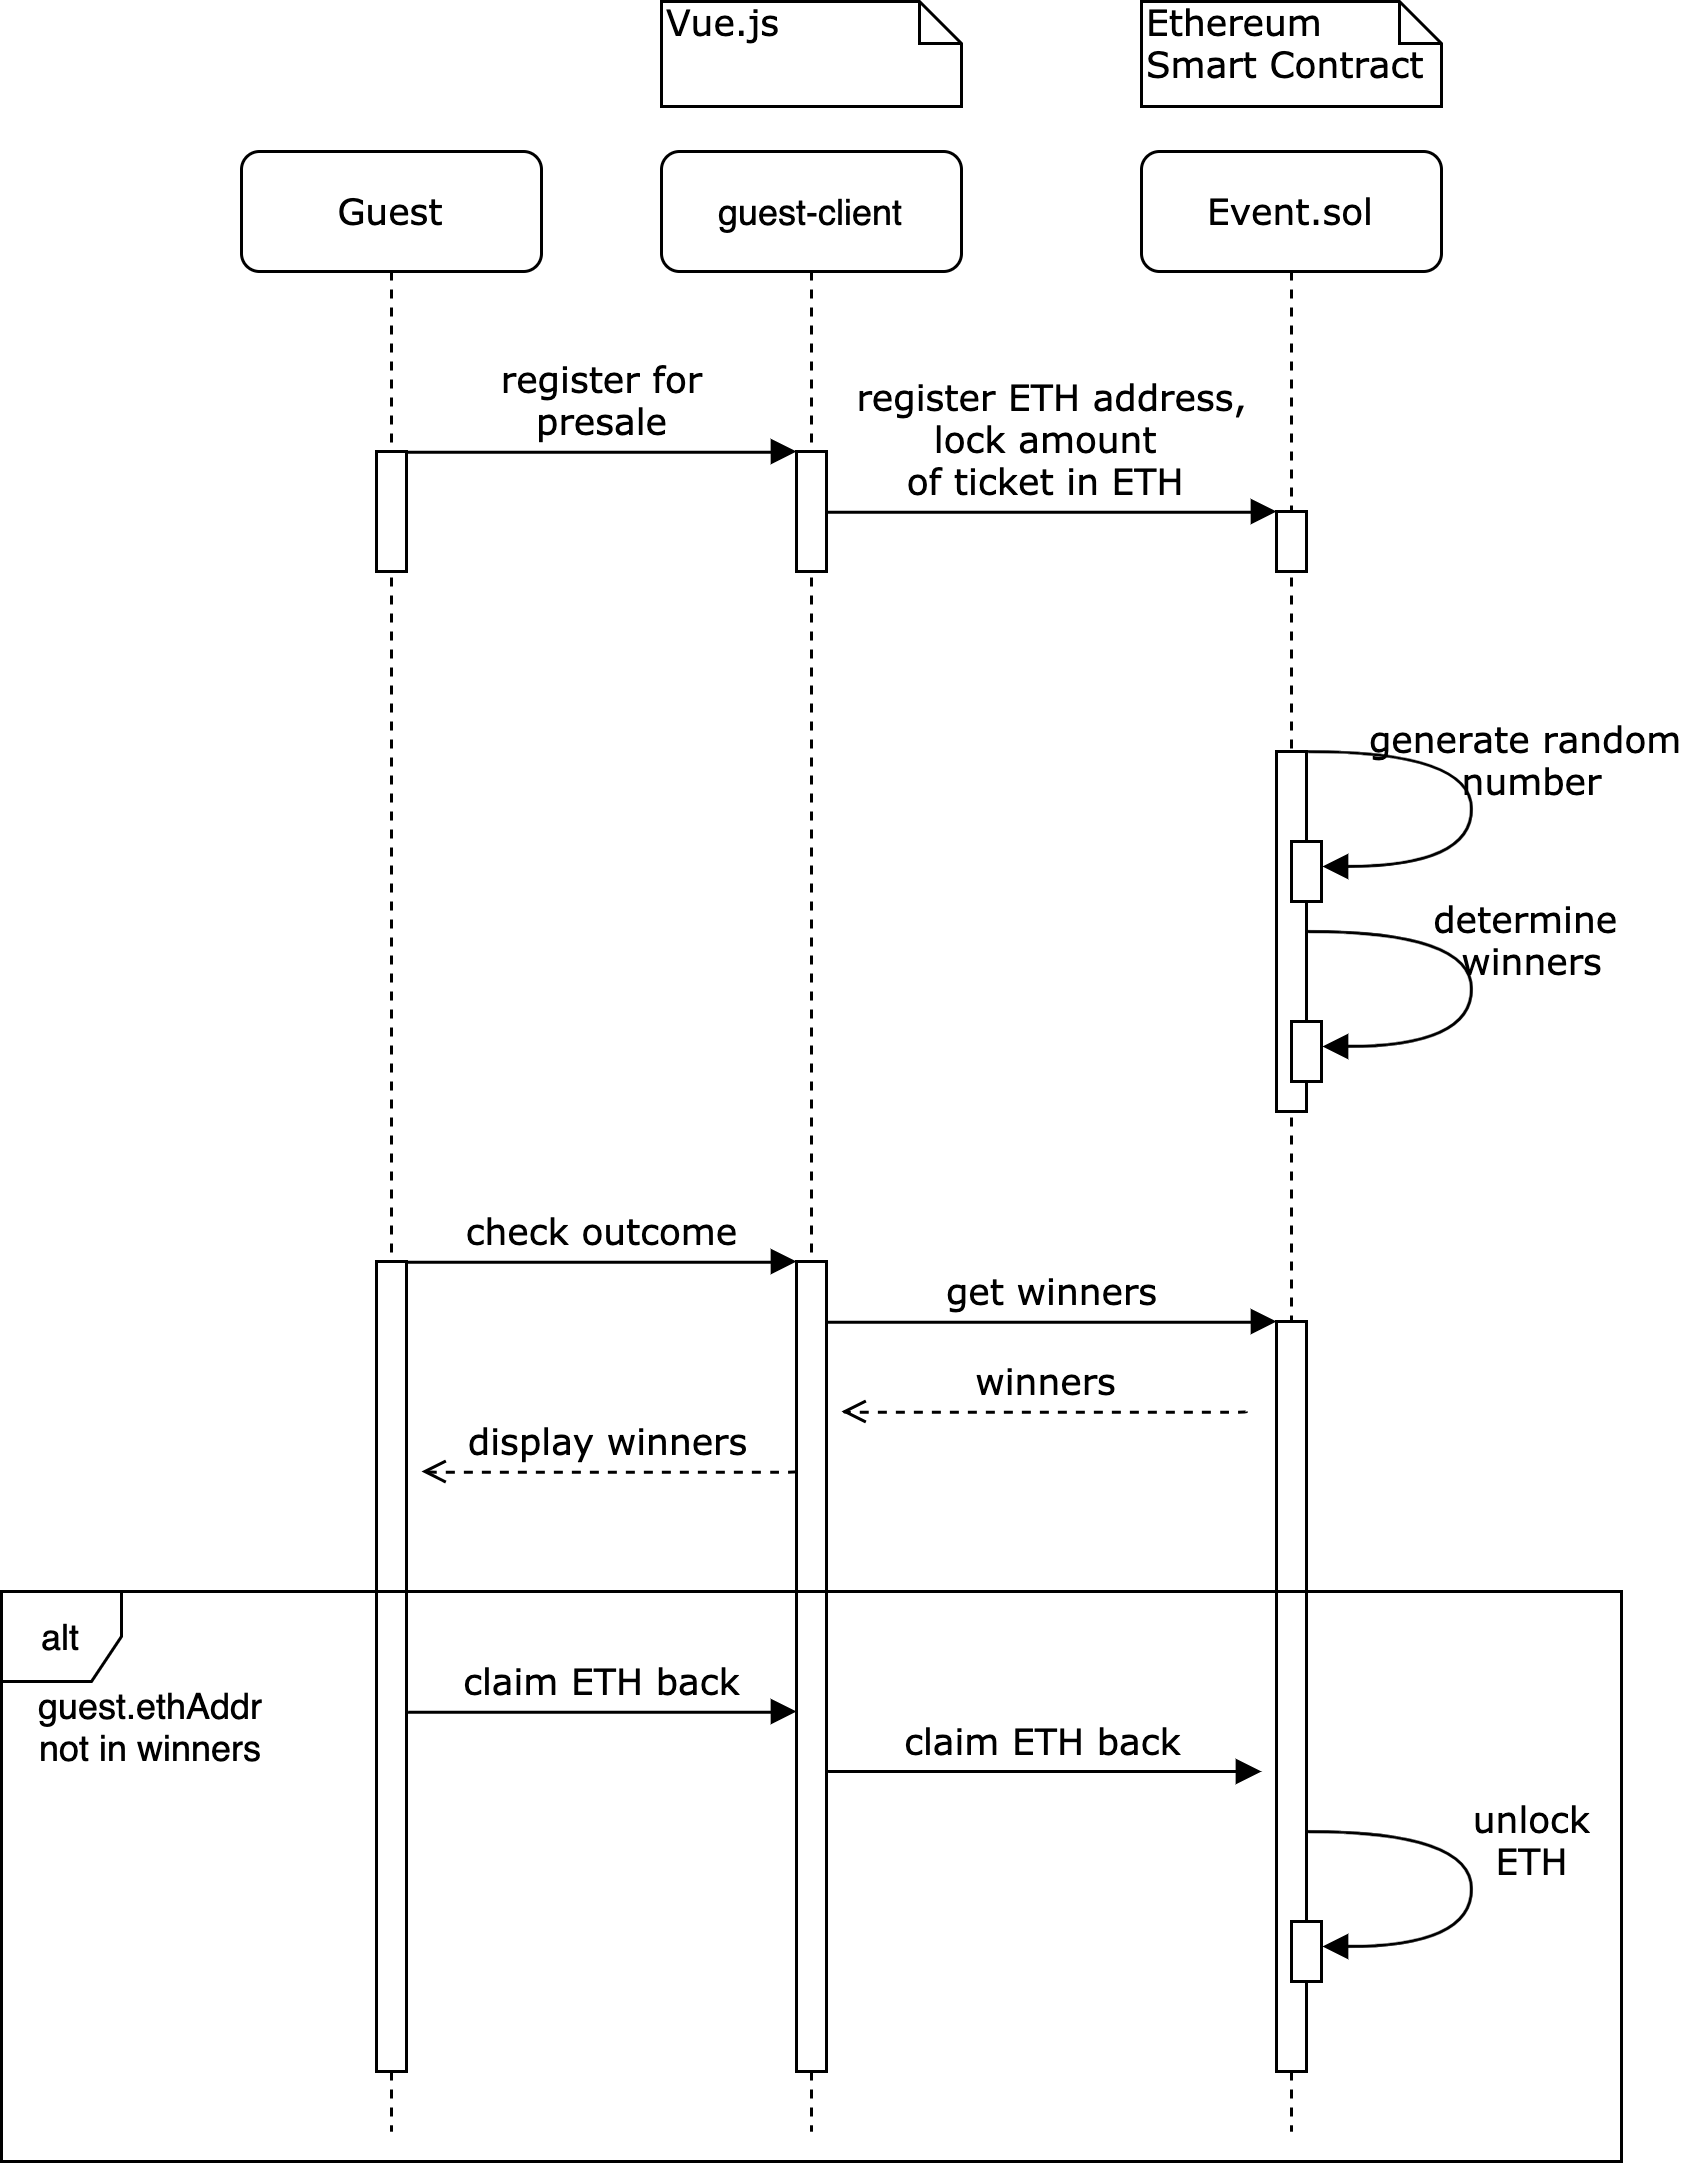
\includegraphics[width=14cm]{design/diagrams/presale.png}
    \caption{Presale Sequence Diagram}
    \label{fig:presale-seuquence-diagram}
\end{figure}

\subsection{Buy a Ticket from an Affiliate Link}
To broaden an event's visibility, a host may want to hire affiliates to promote their event. To do so, the host can register affiliates on the event SC, so that the affiliate can distribute a link containing his Ethereum address as query segment. The buying process is the same as in Figure \ref{fig:buyticket-sequence-diagram}. However, the affiliate's address is also forwarded to the SC and is linked to the bought ticket as well. After the event, when the ticket prices in ETH are unlocked, the affiliate can request to receive the award from each ticket that was sold holding his address as affiliate.
\begin{figure}[H]
    \centering
    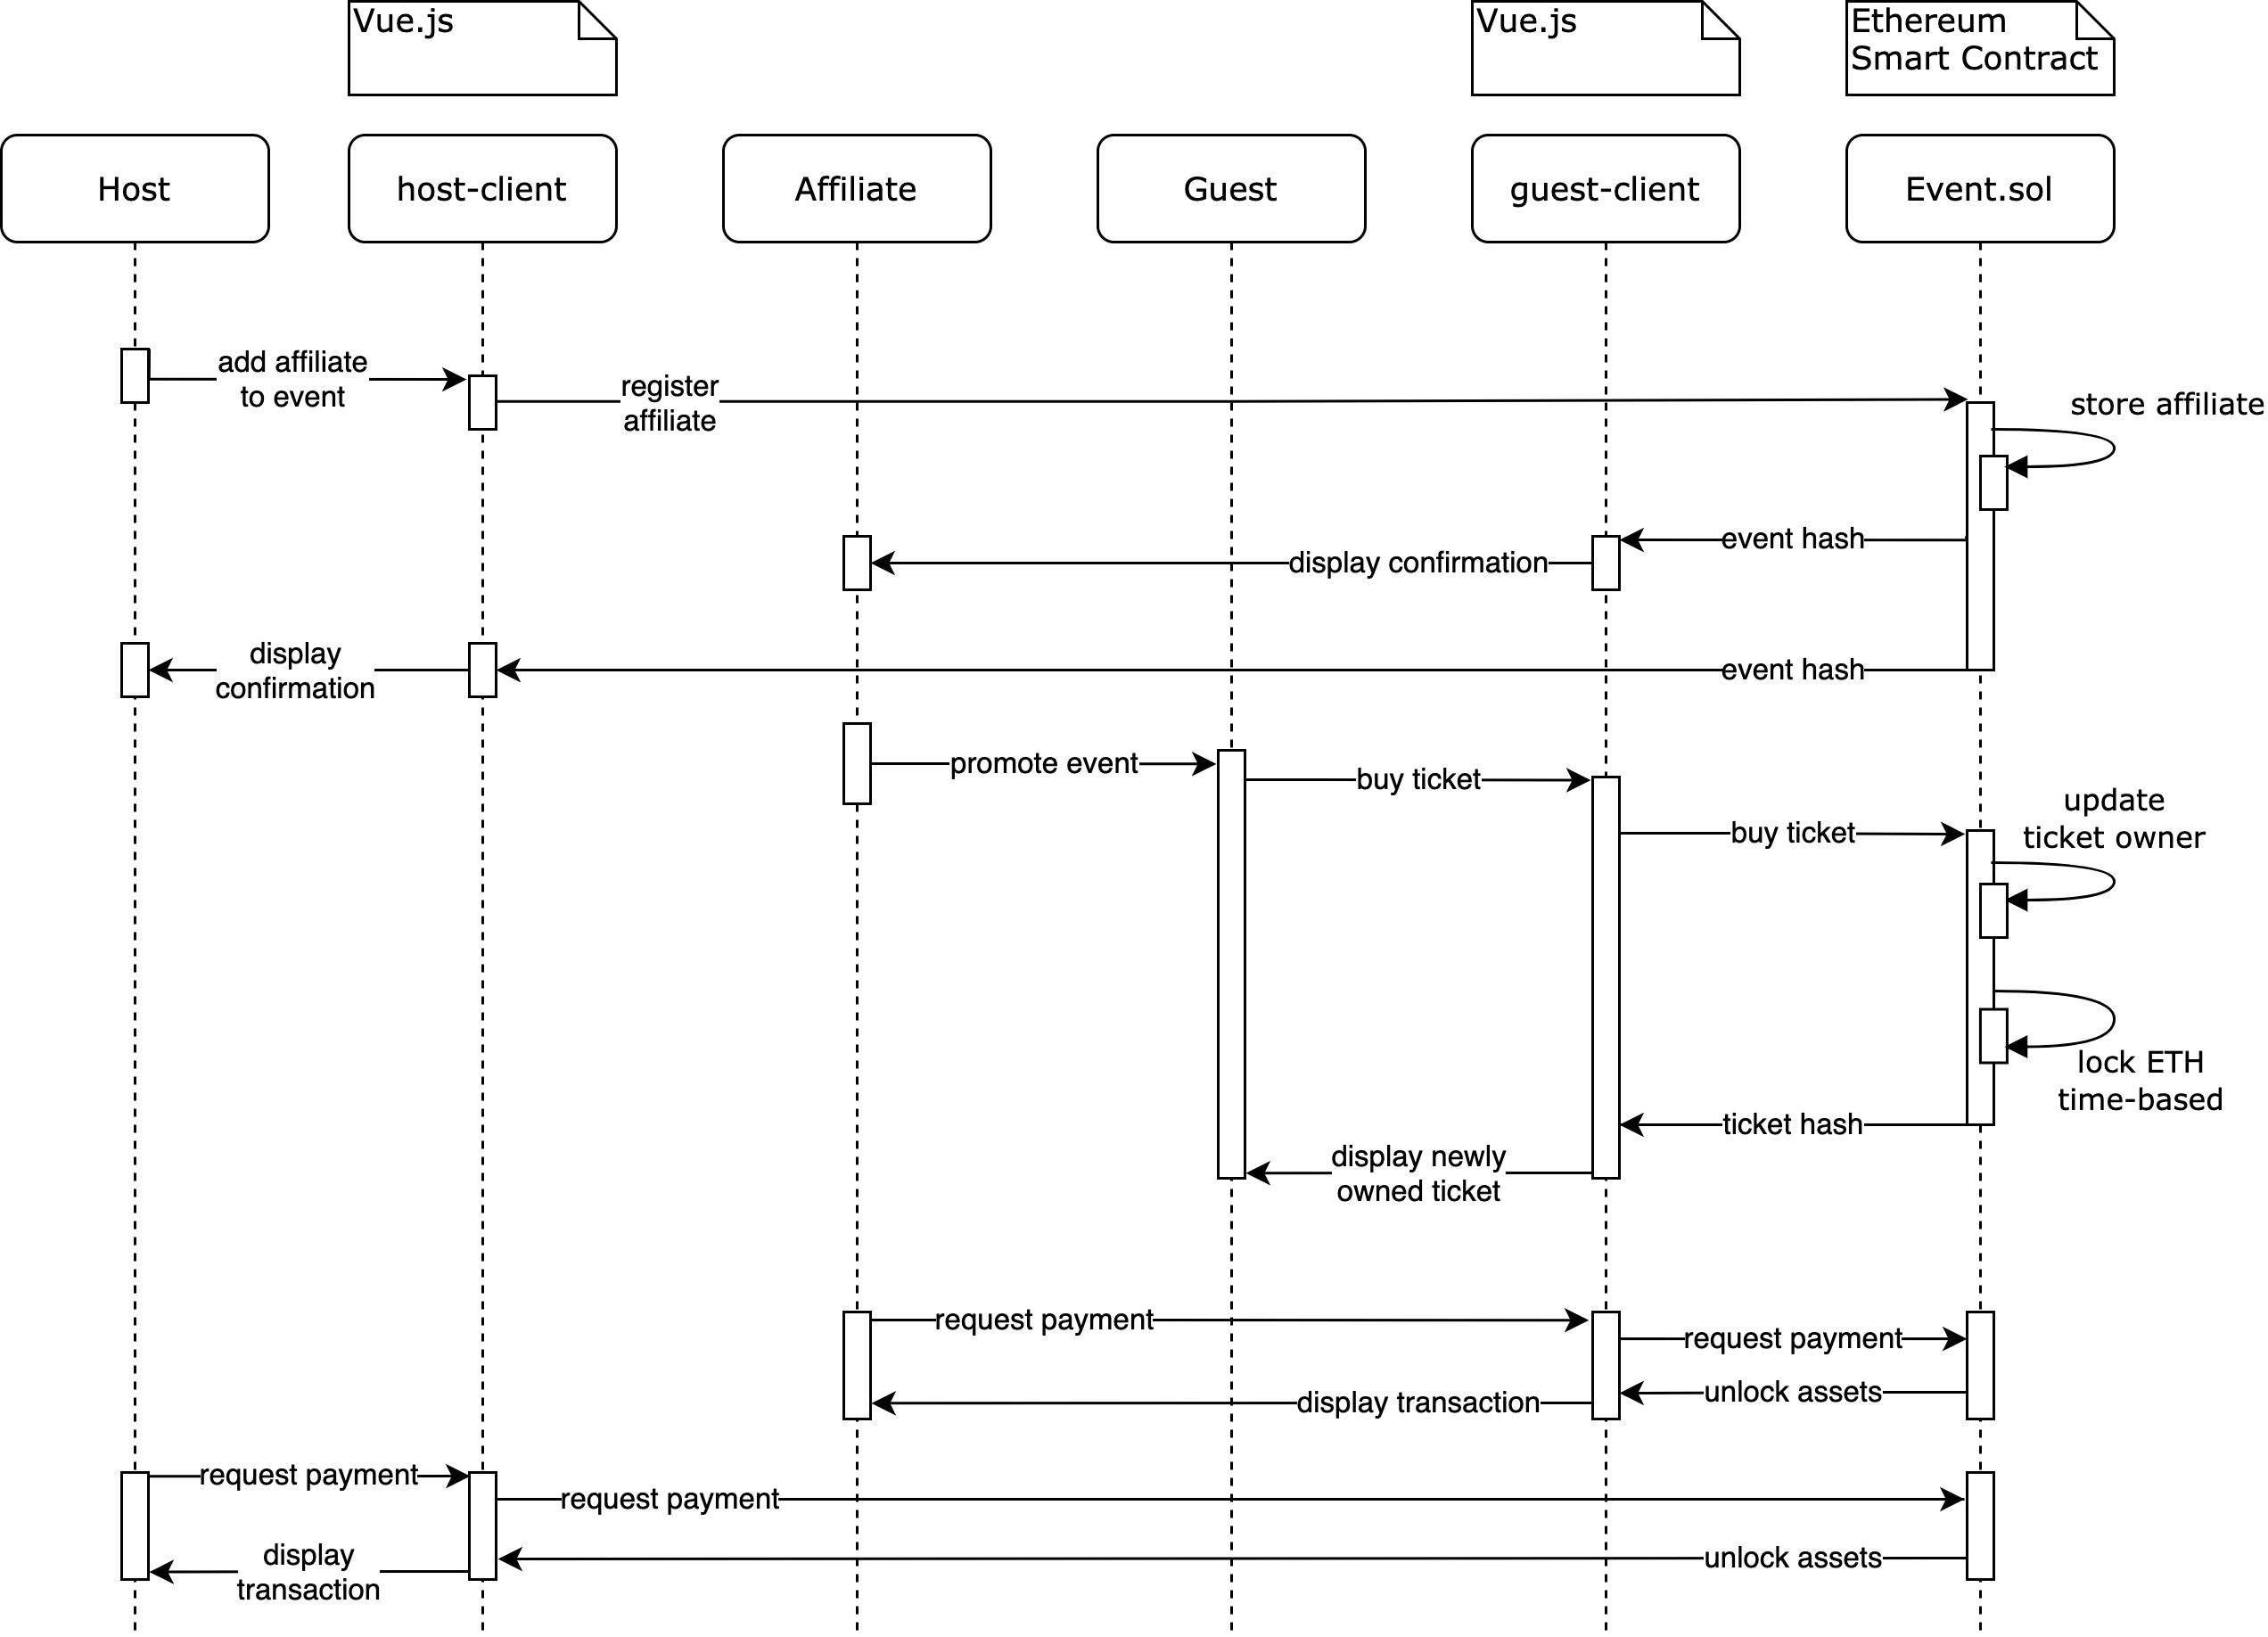
\includegraphics[width=16cm]{design/diagrams/BuyTicketFromAffiliateLink.png}
    \caption{Ticket Sale from Affiliate Link Sequence Diagram}
    \label{fig:buyticket-from-affiliate-diagram}
\end{figure}

\subsection{Identity Registration}
In Switzerland, to get a new phone number, you have to provide your passport details. Therefore a scalper cannot go through the process of approving his identity multiple times. The sequence diagram in Figure \ref{fig:identity-registration-airbnb} illustrates how a guest can prove his ownership of his phone number. To do so, the guest uses the \textit{guest-client} application to register an identity verification request. This request will be forwarded to the \textit{identity-approver} application. The identity approver is a trusted entity that checks if a user is in control of a certain Ethereum address, phone number, etc. In this scenario the user proofs his ownership of a phone number.  The idea of the identity approver is to store the uniqueness characteristic of that phone number and link it to a Ethereum address without the need of creating another KYC process. 

The identity approver generates a random sequence and sends it back to the identity the guest wants to proof ownership of. The guest receives the random sequence and enters it into the guest-client. The guest is then asked to sign the random sequence using his Ethereum address. The \textit{identity-approver} checks the signature for its validity. If this check completes successfully, a proof is generated.

Important to note is that the \textit{identity-approver} is a trusted entity. However, the goal is to build an application that does not rely on a single trusted entity. Thus, a system is envisioned where an event host can select from different identity approver and providers. It should even be possible that an event host can also act as the identity provider and approver. This would make sense for a large event company that want to make sure that no fraud is made by third parties. 

\begin{figure}[H]
    \centering
    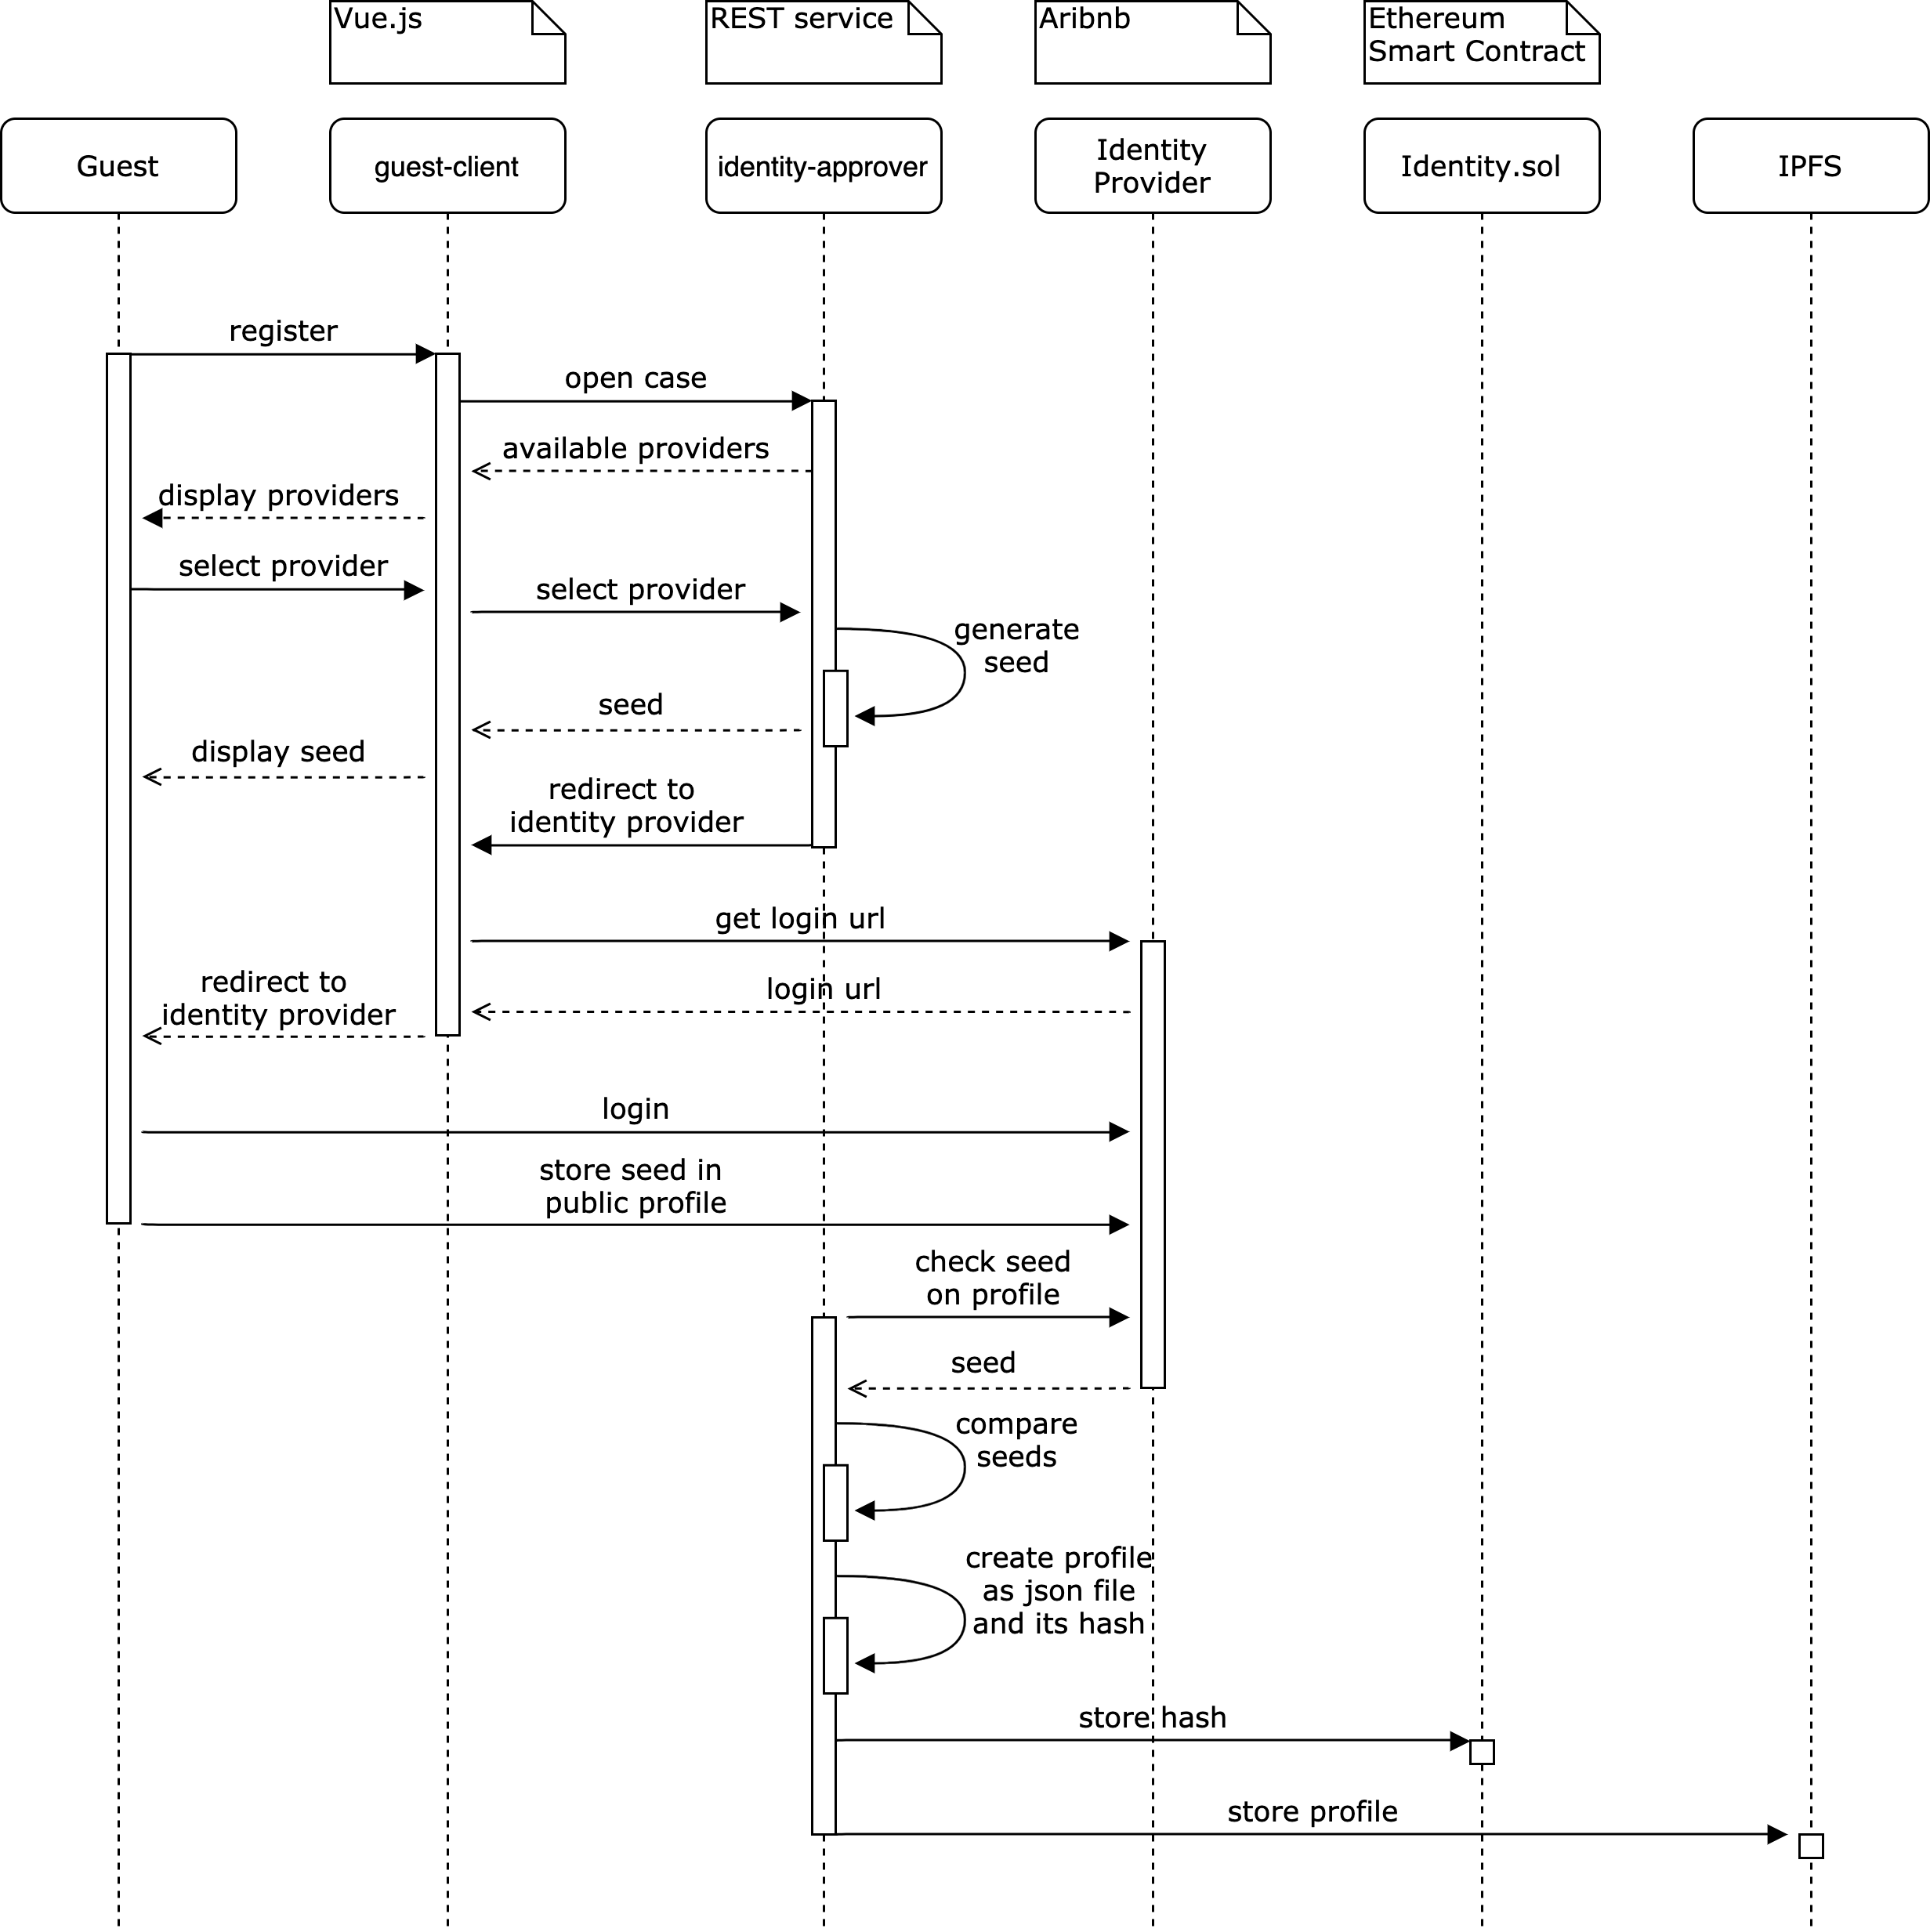
\includegraphics[width=16cm]{design/diagrams/identy-registration-airbnb.png}
    \caption{Identity Registration Phone number}
    \label{fig:identity-registration-airbnb}
\end{figure}

\subsection{Resell Ticket}
The guest logs into his account. The guest-client the gets all the Tickets owned by the guest, that are still valid. It then retrieves the ticket metadata form the IPFS storage. After the metadata has been retrieved, the guest gets shown the ticked owned by him. the guest then chooses the ticket he does no longer want to have and therefore selects the option to sell his ticket in the guest-client. This lists the ticket on the aftermarket. Whenever the ticket is bought by another guest, the money used to buy the ticket is directly transferred to the wallet of the seller of the ticket. When the guest checks his balance again, he will see the added funds.

This process is illustrated in the following sequence diagram.

\begin{figure}[H]
    \centering
    \includegraphics[width=16cm]{design/diagrams/Resell Ticket.png}
    \caption{Resell ticket}
    \label{fig:Resell-ticket}
\end{figure}

 


\subsection{Buy Ticket From Reseller}
\begin{figure}[H]
    \centering
    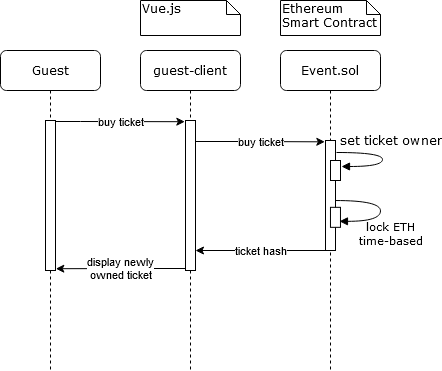
\includegraphics[width=12cm]{design/diagrams/BuyTicketFromResell.png}
    \caption{Buy Ticker from reseller}
    \label{fig:buyFromResell}
\end{figure}
The process of buying a ticket from the resell market looks exactly the same as buying directly from the host directly from the customers point-of-view, as depicted in \ref{fig:buyFromResell}. The Guest first connects to his wallet through his private key on the guest web application. Then he selects the event he is interested in and chooses to buy a ticket, which invokes the corresponding SC. Exactly as seen in \ref{fig:buyticket-sequence-diagram}, the SC locks the price of the ticket until the event has passed and returns the ticket hash to the guest web application, where it is displayed to the guest.

\subsection{Access Control}\label{subsection:access-control}

\begin{figure}[H]
    \centering
    \includegraphics[width=16cm]{design/diagrams/AcessControl.png}
    \caption{Access Control Sequence Diagram}
    \label{fig:access-controll}
\end{figure}

As the guest wants to gain access to the event, he is confronted with the entrance control. As the ticket is linked to the Ethereum address of the guest, he just has to prove the ownership of the given Ethereum address. In order to do this, the guest has to provide a signature of a message. This signature together with the message and the guest's public address can then be verified which ultimately proves that the guest owns this Ethereum address.

For this process three components are necessary. First of all, access terminal web applications (see section \ref{design:access-terminal}) are intended to run on tablet at the venue. They are used to display messages to be signed, a backend is needed to handle the signatures and keeping track of the state of the terminals and an embedded camera feature in the guest client application is required to scan the information from the terminal, sign the message and sending the signature to the backend for verification.

%Access terminals are placed at the respective entrances to display messages to be signed. A backend spring application provides an API to register terminals, create new messages for signing, verify signatures and check whether a ticket of the guest actually exists and was not already used to enter the event. 

%Access Terminals (see Subsection \ref{design:access-terminal}) are placed at the respective entrances. These terminals have to be registered with a secret code stored in the backend. When a terminal is registered, it is allocated a unique random sequence, which is stored in the backend and in the terminal application.

The entrance control terminals (see Subsection \ref{design:access-terminal}) are registered at the backend. Every terminal gets its unique identifier. The terminal then requests a unique random sequence, which is stored with the corresponding terminal id in the backend. This random sequence is then displayed alongside the backend URL as a QR-code on the terminal. The guest reads the QR-Code and extracts the random sequence. He then proceeds to sign the sequence using his Ethereum address proofing his ownership. The signature, the Ethereum address, the number of tickets he wants to use and the random sequence are then sent to the backend. The backend then evaluates the validity of the signature. After that, it is checked, whether the random sequence exists and the block chain is queried, to check, whether the Ethereum address actually holds enough tickets. It is also checked, whether this ticket already entered the venue. When all these checks are successful, the terminal, specified by its id, is messaged to let the guest pass. At the same time, the Ethereum address and the corresponding ticket are added to the database, that tracks the area the ticket owner are in. This implementation also holds for changing from different areas in a venue, for example accessing the VIP are from the general area of the venue.


%\begin{figure}[H]
%    \centering
%    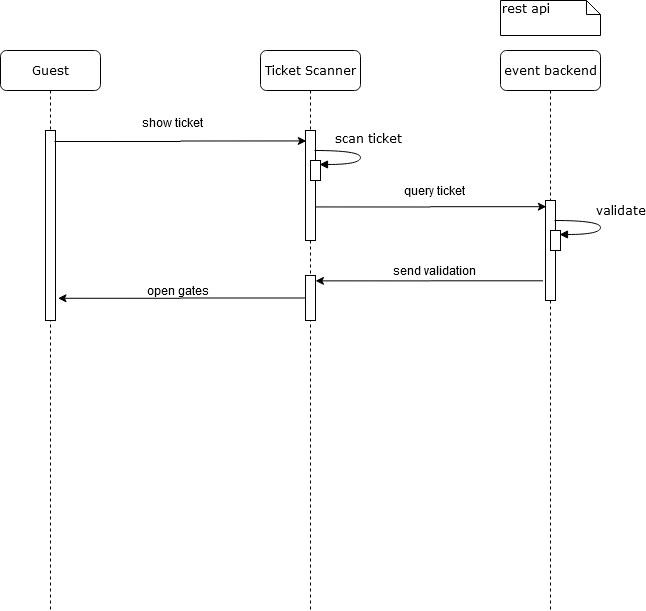
\includegraphics[width=14cm]{design/diagrams/entrance.png}
%    \caption{Entrance Control}
%    \label{fig:entranceControl}
%\end{figure}

%The sequence diagram in \ref{fig:entranceControl} depicts the process applied at the event gates for handling entrance control. The guest presents his ticket to the employee at the gate in form of a QR-code on his phone. The employee scans the code using the ticket scanner mobile application, which invokes a call to the rest API on the event backend, which contains a database with all tickets and the public keys of their respective owners. Once the Ticket Scanner application receives the confirmation from the server that the code is valid, the guest is granted access to the event.



% \subsection{Event Cancellation}
%This Section demonstrates how a guest can issue a report if an event was fraudulent or did not take place and the event host did not pay back the ticket price. 

%The sequence diagram in Figure \ref{fig:dispute-resolution-approved} shows how a guest rightfully reports a dispute and in Figure \ref{fig:dispute-resolution-rejected} the guest is not entitled to issue a dispute. 

%When the host creates an event, a fixed amount of ETH is locked as a deposit as well as a trusted third party is used to verify the guest's identification as explained in Figure \ref{fig:identity-registration-airbnb}. This party also acts as a dispute resolver. It is envisioned that this entity consists of multiple parties but for simplicity reasons it is shown as one ETH account. The deposit is locked until the challenge period is over. During the challenge period a guest can report fraudulent events.

%When the dispute resolver receives examination requests, they contact the event host for access proof. These proofs can only be generated by the ticket holders and contain the event id and the date of access. If the host can provide such requests, the tickets were used to enter the venue. The claim that the event was fraudulent is wrong and the host deposit will be unlocked for the host when the challenge period is over. 


%\begin{figure}[H]
%    \centering
%    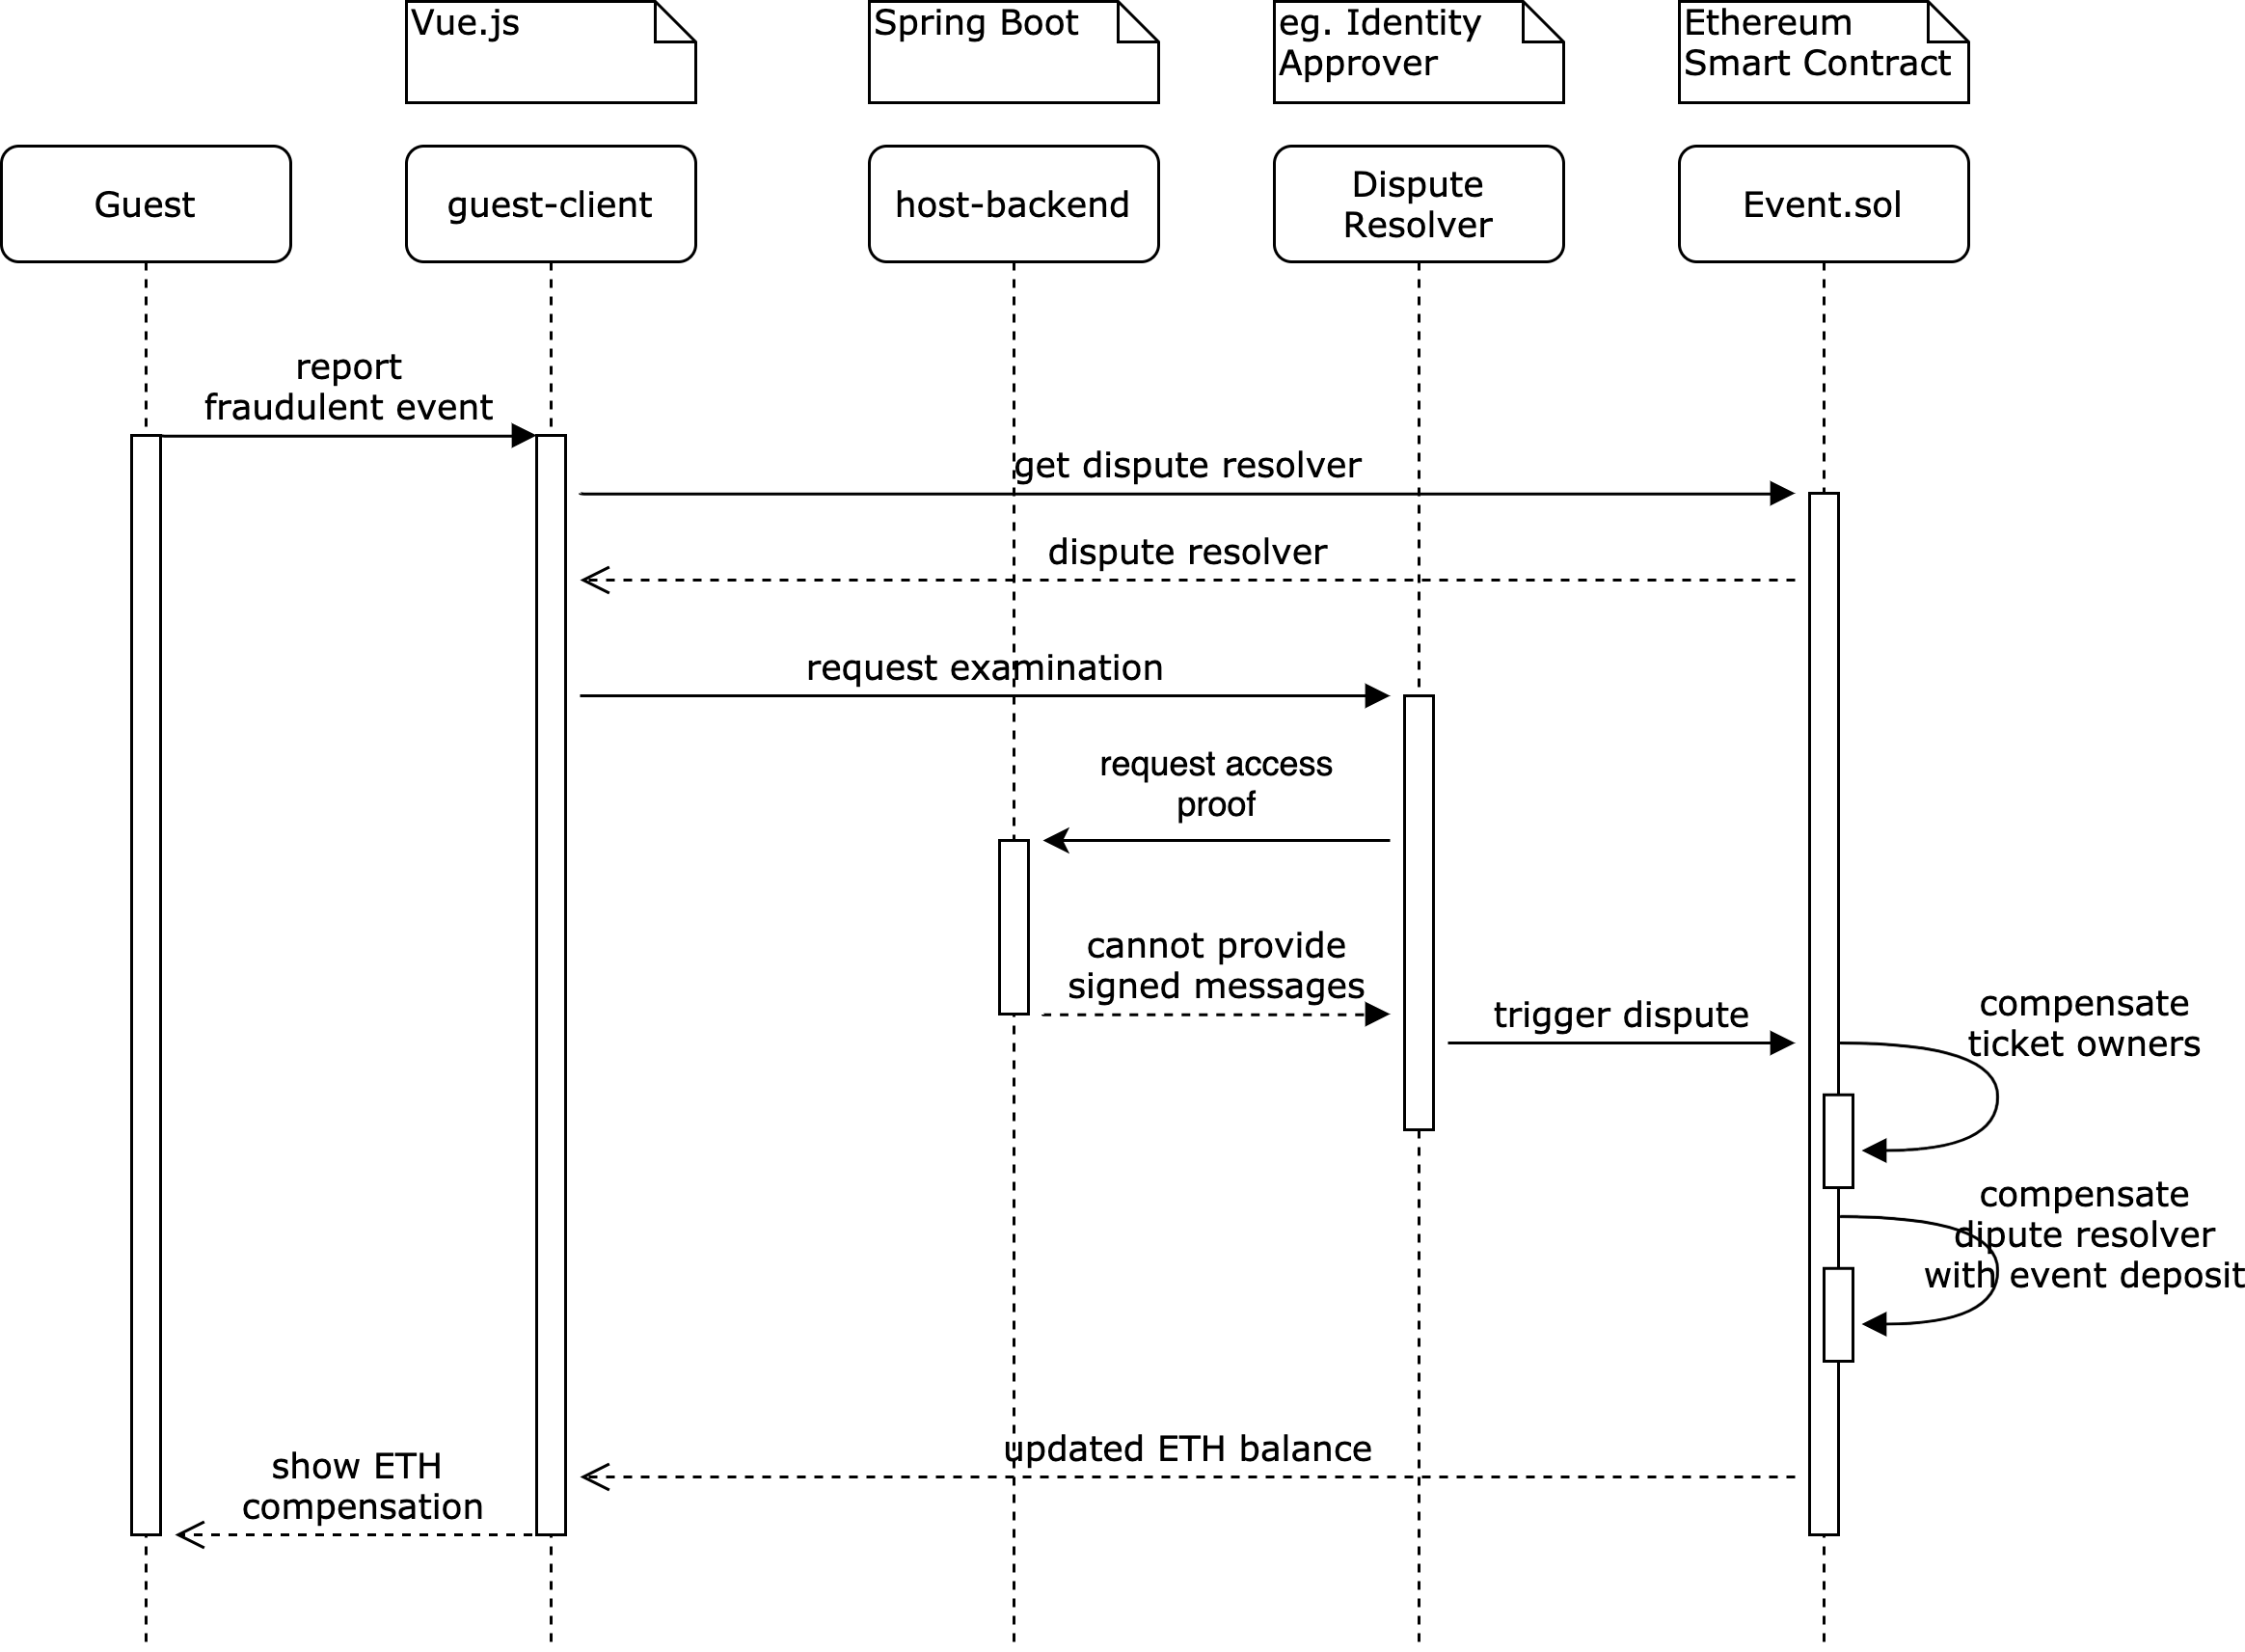
\includegraphics[width=16cm]{design/diagrams/dispute-resolution-approved.png}
%    \caption{Event Cancellation Approved}
%    \label{fig:dispute-resolution-approved}
%\end{figure}


%In the case where the event is fraudulent, the event host cannot provide signed proofs that tickets were used to enter the venue. The dispute resolver then calls the SC to send the locked ETH in the SC back to the ticket owners. Also the dispute resolver is compensated with the deposit that the event host initially had to deposit when the event was created. 

%\begin{figure}[H]
%    \centering
%    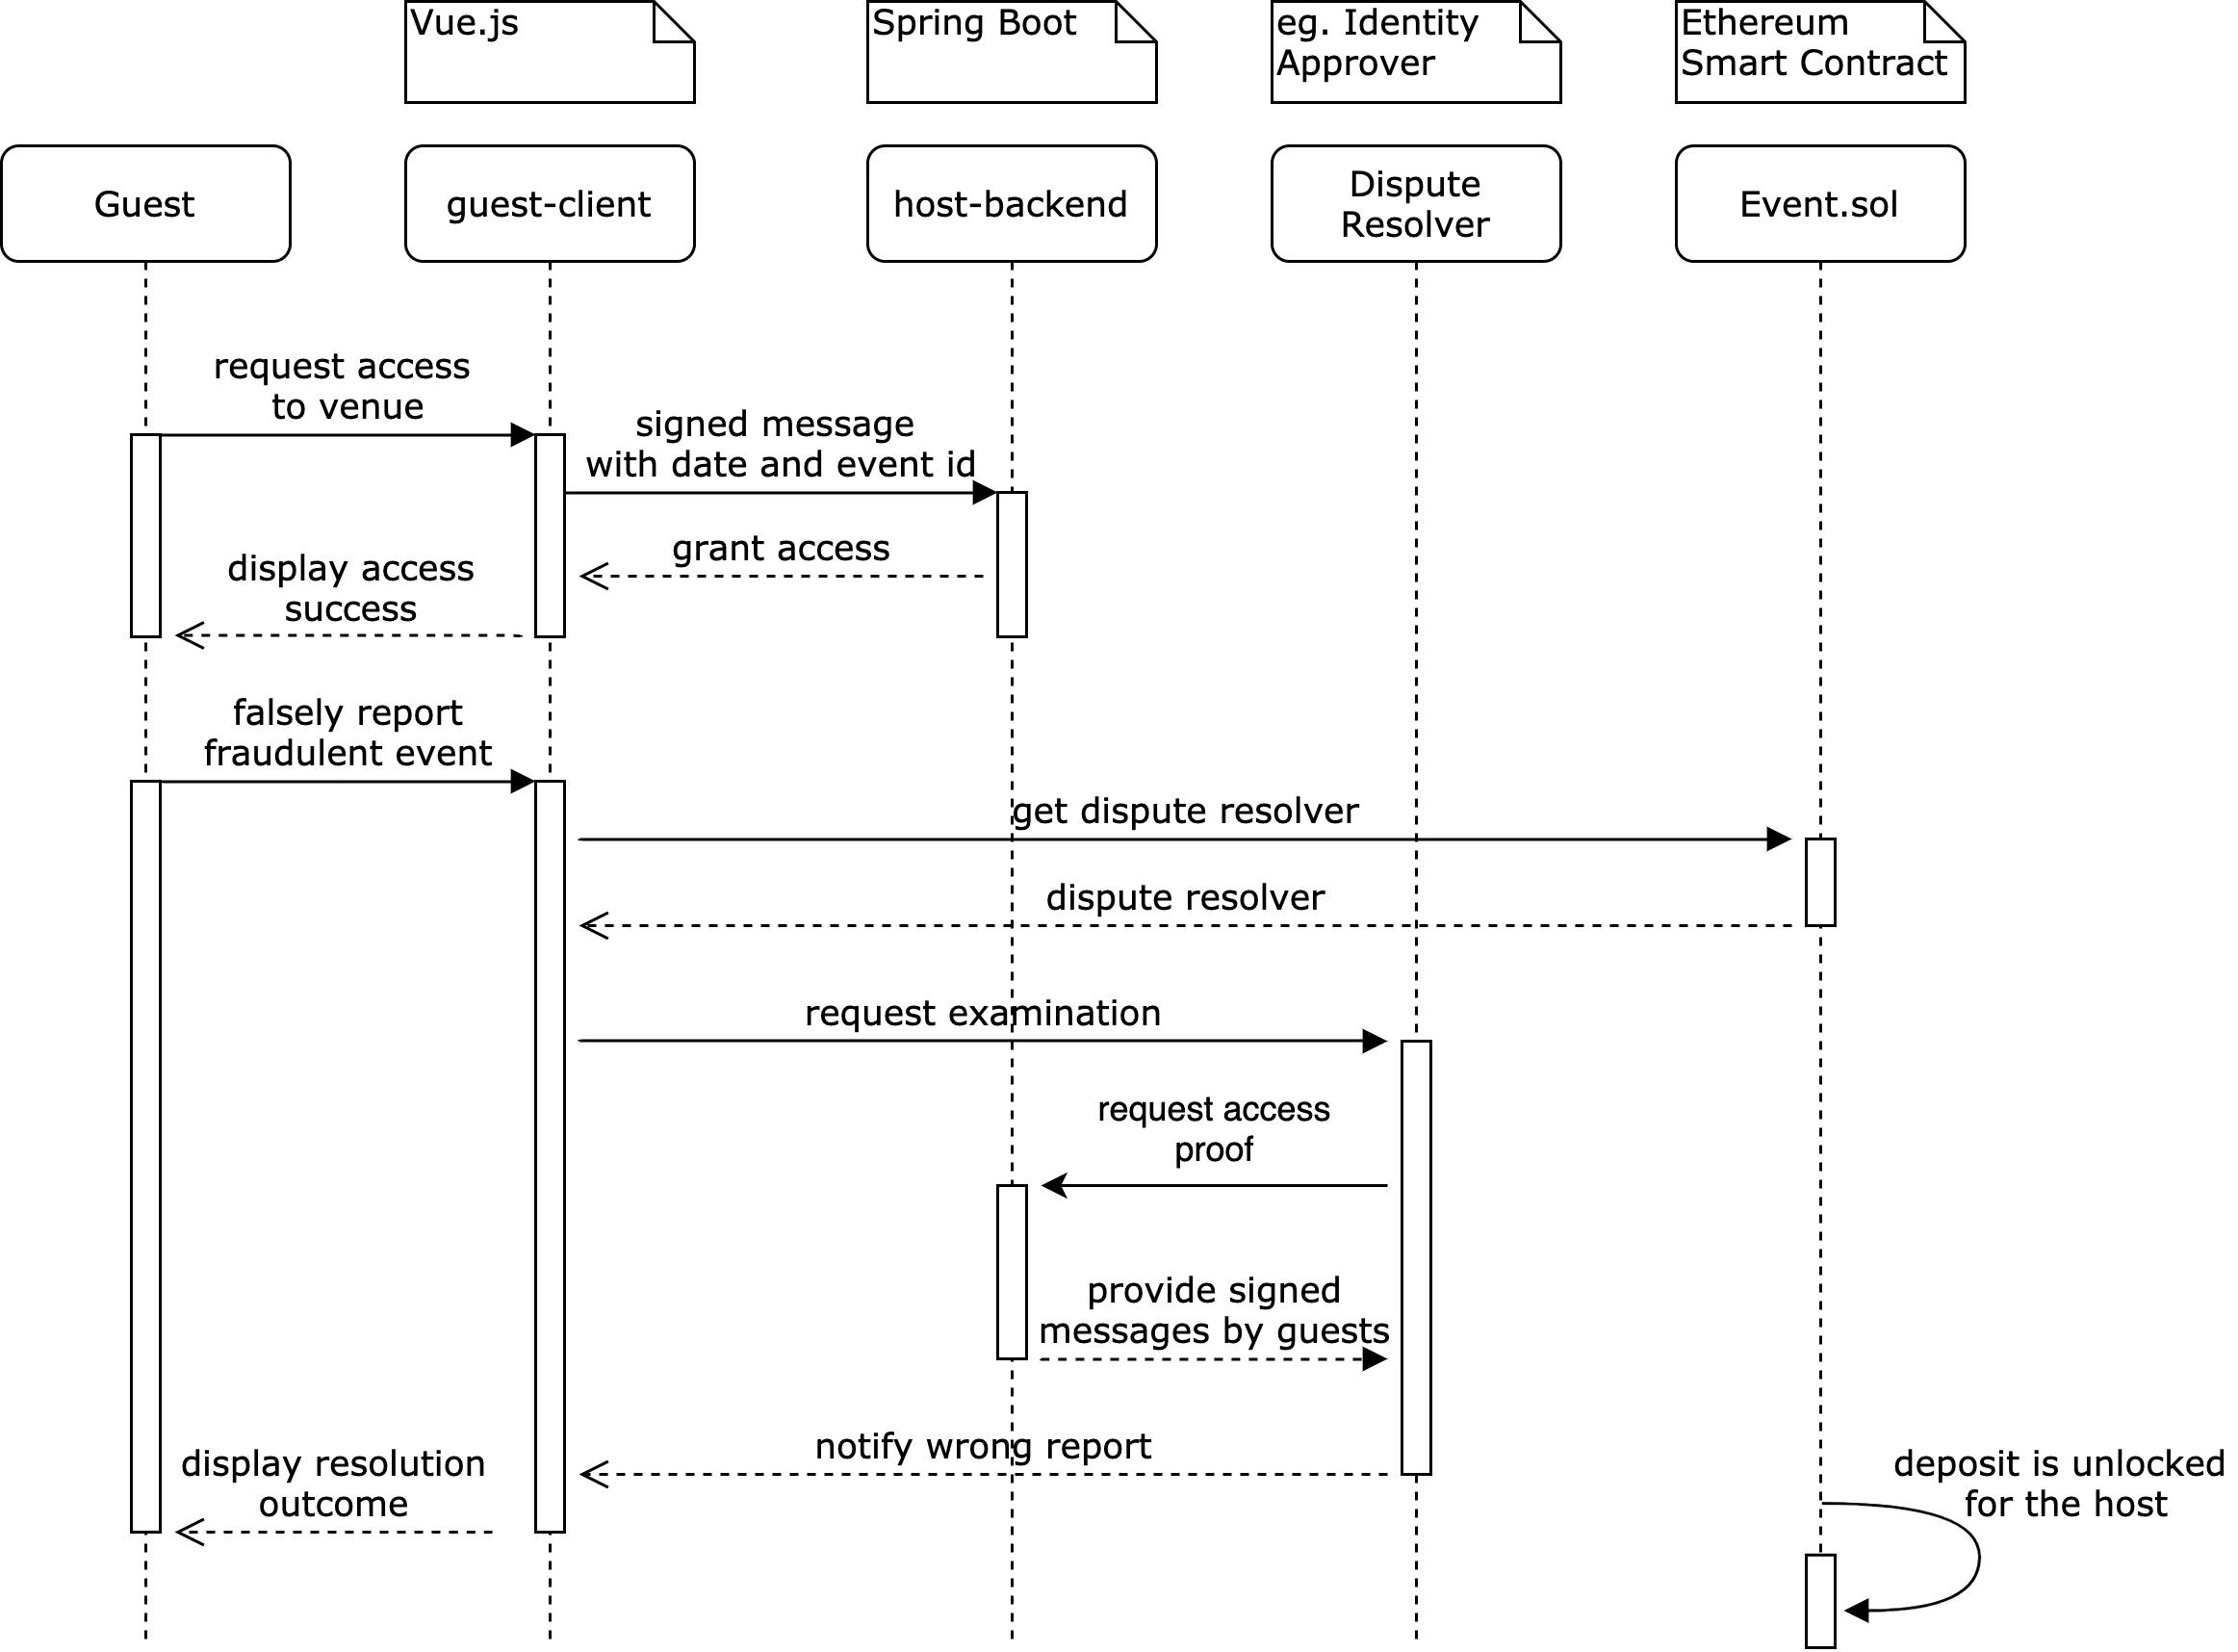
\includegraphics[width=16cm]{design/diagrams/dispute-resolution-rejected.png}
%    \caption{Event Cancellation Rejected}
%    \label{fig:dispute-resolution-rejected}
%\end{figure}